\documentclass[aspectratio=169,9pt]{beamer}
\usetheme{Warsaw}
\usepackage{amsmath,amssymb,booktabs,tabularx,colortbl}
\usepackage{graphicx}
\usepackage{tikz}

% ── Macros ──────────────────────────────────────────────────────────────────
\newcommand{\figdir}{figs}
\newcommand{\anafig}[1]{\figdir/#1}
\newcommand{\sigIQR}{\sigma_{\mathrm{IQR}}}
\newcommand{\sigG}{\sigma_{\mathrm{G}}}
\newcommand{\NEND}{N_{\mathrm{END}}}
\newcommand{\NTOP}{N_{\mathrm{TOP}}}
\newcommand{\NTOT}{N_{\mathrm{total}}}
\newcommand{\Tblue}{T_{\mathrm{BLUE}}}
\newcommand{\TEND}{T_{\mathrm{END}}}
\newcommand{\TTOP}{T_{\mathrm{TOP}}}
\newcommand{\wend}{w_{\mathrm{END}}}
\newcommand{\wtop}{w_{\mathrm{TOP}}}
\newcommand{\rhoET}{\rho_{\mathrm{ET}}}
\newcommand{\sEND}{\sigIQR(\TEND)}
\newcommand{\sTOP}{\sigIQR(\TTOP)}
\newcommand{\sBLUE}{\sigIQR(\Tblue)}
\newcommand{\ps}{\ensuremath{\,\mathrm{ps}}}
\newcommand{\ns}{\ensuremath{\,\mathrm{ns}}}
\newcommand{\mm}{\ensuremath{\,\mathrm{mm}}}
\newcommand{\MeV}{\ensuremath{\,\mathrm{MeV}}}
\newcommand{\mmns}{\ensuremath{\,\mathrm{mm/ns}}}

% ── Colours ─────────────────────────────────────────────────────────────────
\definecolor{azblue}{rgb}{0.0,0.45,0.70}
\definecolor{orng}{rgb}{0.85,0.55,0.0}
\definecolor{grn}{rgb}{0.0,0.50,0.10}
\setbeamercolor{alerted text}{fg=red!70!black}

% ── Presenter ───────────────────────────────────────────────────────────────
\title[SHiP Timing Bar]{From first principles to optimised readout\\
  of a SHiP timing bar}
\subtitle{Photon transport, order-statistic estimators, and BLUE combination}
\author{R.~Ríos Pino}
\institute{SHiP Collaboration / CINVESTAV}
\date{August 2026}

\setbeamertemplate{navigation symbols}{}
\setbeamertemplate{footline}[frame number]
\setbeamertemplate{headline}{}  % suppress Warsaw nav balls (too many slides → overfull)

% ── Helpers ─────────────────────────────────────────────────────────────────
\newcommand{\hl}[1]{\textcolor{azblue}{\textbf{#1}}}
\newcommand{\hlr}[1]{\textcolor{red!70!black}{\textbf{#1}}}
\newcommand{\hlo}[1]{\textcolor{orng}{\textbf{#1}}}
\newcommand{\hlg}[1]{\textcolor{grn}{\textbf{#1}}}

\begin{document}

%===============================================================================
\frame{\titlepage}

%===============================================================================
\begin{frame}{One bar, $\sim$600 bars, one timing system}
\begin{columns}[T]
\column{0.48\textwidth}
\textbf{Geometry of a single bar}
\begin{itemize}
  \item Scintillator: $1400\times60\times10\,\mathrm{mm}^3$
  \item END readout: \hl{8~SiPMs/end $\times$ 2~ends = 16 total}
  \item TOP readout (hybrid): \hlo{20 SiPMs} sparse along top face
  \item Hybrid total: $\NEND{=}16 + \NTOP{=}20 = \NTOT{=}36$
\end{itemize}
\vspace{4pt}
\textbf{Detector scale}
\begin{itemize}
  \item Bar area $\approx 1.4\times0.06 = 0.084\,\mathrm{m}^2$
  \item Full detector $\approx 50\,\mathrm{m}^2$ $\Rightarrow$ $\sim600$ bars
  \item $\NTOT = 36 \Rightarrow \sim\!21\,600$ channels total
  \item Each saved SiPM per bar removes $\sim600$ channels
\end{itemize}
\column{0.48\textwidth}
\vspace{6pt}
\textbf{Design question} (not merely "smallest $\sigma$"):
\begin{alertblock}{}
What is the \emph{minimum practical} instrumentation
that delivers event time AND position for each bar?
\end{alertblock}
\vspace{4pt}
Figures of merit:
\begin{itemize}
  \item Timing resolution $\sigma_t$
  \item Longitudinal position $\sigma_x$
  \item Response uniformity along bar
  \item Channel count
  \item Robustness to SiPM/electronics jitter
\end{itemize}
\end{columns}
\end{frame}

%===============================================================================
\begin{frame}{Strategy: napkin first, Geant4 second}
\begin{columns}[T]
\column{0.5\textwidth}
\textbf{Why an analytic model?}
\begin{itemize}
  \item Builds physical intuition before simulation
  \item Sets order-of-magnitude expectations
  \item Diagnoses surprises in Geant4 output
  \item Identifies dominant parameters
\end{itemize}
\vspace{4pt}
\textbf{Chain}
{\footnotesize\[
  \mu \xrightarrow{\mathrm{L}} E_{\mathrm{dep}}
  \to N_\gamma \to f_{\mathrm{TIR}}
  \to P_{\mathrm{surv}} \to N_{\mathrm{pe}}
\]}
\column{0.46\textwidth}
\begin{block}{Crucial distinction}
  The napkin gives \emph{scales and trends}.
  Agreement at $\sim20\%$ level is a success,
  not a precision measurement.
\end{block}
\vspace{6pt}
\textbf{This talk}
{\small\begin{enumerate}
  \item First-principles photon transport
  \item Geant4 validation / photon budget
  \item Estimator optimisation
  \item Position reconstruction
  \item Detector design outlook
\end{enumerate}}
\end{columns}
\end{frame}

%===============================================================================
\begin{frame}{Energy deposition: $\sim\!2\MeV$ from a 1\,GeV $\mu^-$}
\begin{columns}[T]
\column{0.50\textwidth}
For a minimum-ionising particle in plastic ($\rho\approx 1.03\,\mathrm{g/cm}^3$):
\[
  \left\langle\frac{dE}{dx}\right\rangle \approx 2\,\mathrm{MeV/cm}
\]
Bar thickness along muon track: $T = 1\,\mathrm{cm}$ (vertical incidence)
\[
  E_{\mathrm{dep}} \approx 2\MeV \quad \text{(Landau peak)}
\]
The Landau distribution has a \emph{tail} to high values;
the napkin uses only the most probable value.

\column{0.46\textwidth}
\begin{alertblock}{Simulation input}
  Geant4 uses the full Landau distribution
  event-by-event.
  The $\sim\!2\MeV$ scale is confirmed by the simulation;
  event-by-event fluctuations in $N_\gamma$ propagate
  into the timing residuals.
\end{alertblock}

\vspace{6pt}
\textbf{Practical consequence}: photon number varies
event-by-event (Landau + Poisson), broadening the
timing distribution beyond pure photon statistics.
\end{columns}
\end{frame}

%===============================================================================
\begin{frame}{Photon production: $N_\gamma \approx 1.9\times10^4$ per muon}
\begin{columns}[T]
\column{0.52\textwidth}
For EJ-230 (scintillation yield $Y = 9700\,\mathrm{photons/MeV}$):
\[
  N_\gamma = Y \cdot E_{\mathrm{dep}} = 9700 \times 2 \approx 1.9\times10^4
\]
All three materials for comparison:

\smallskip
{\small
\begin{tabular}{lccc}
\toprule
Material & Yield & $\tau$ & $\lambda_{\mathrm{att}}$ \\
         & [ph/MeV] & [ns] & [mm] \\
\midrule
EJ-200 & 10\,000 & 2.1 & 3800 \\
EJ-204 & 10\,400 & 1.8 & 1600 \\
EJ-230 & 9\,700  & 1.5 & 900  \\
\bottomrule
\end{tabular}}

\vspace{6pt}
\textbf{Napkin prediction}: EJ-230 wins timing
despite fewer photons, because shorter $\tau$
provides earlier peak arrival.

\column{0.44\textwidth}
\includegraphics[width=\linewidth]{\anafig{figM2_mat_npe.pdf}}
\vspace{-4pt}
{\footnotesize Geant4: $N_{\mathrm{pe}}/\mathrm{end}$ vs $x$, END + Vikuiti.
EJ-200 $>$ EJ-204 $>$ EJ-230 in photon count — matches napkin.}
\end{columns}
\end{frame}

%===============================================================================
\begin{frame}{TIR: which directions reach an end face?}
\begin{columns}[T]
\column{0.50\textwidth}
Critical angle for plastic--air interface ($n=1.58$):
\[
  \theta_c = \arcsin\!\left(\frac{n_{\mathrm{air}}}{n}\right) \approx 39.3^\circ
\]
For one transverse wall family, fraction with $|\cos\theta_\perp| < \cos\theta_c$:
\[
  a = \cos\theta_c \approx 0.774 \quad \text{(single wall)}
\]
For the \emph{rectangular bar} (two independent transverse families):
\[
  f_{\mathrm{TIR}} = 2a - 1 \approx 0.548
\]
Then approximately half propagates toward each end:
\[
  f_{\mathrm{TIR,end}} \approx 0.274
\]

\column{0.46\textwidth}
\begin{alertblock}{Important distinctions}
\begin{itemize}
  \item $2a-1$ is for the \emph{rectangular bar} (two wall families simultaneously)
  \item This is \textbf{not} the Knoll slab result (single wall)
  \item The old $\approx80\%$ referred to a different quantity/geometry; not directly comparable
  \item The napkin uses $f_{\mathrm{TIR,end}} \approx 0.274$
\end{itemize}
\end{alertblock}
\vspace{4pt}
{\small Coverage per end: $8\times6\times6/(60\times10) \approx 0.48$ —
geometric scale estimate only; real acceptance differs.}
\end{columns}
\end{frame}

%===============================================================================
\begin{frame}{Photon propagation: $v_g \approx c/n$ and position tagging}
\begin{columns}[T]
\column{0.50\textwidth}
Group velocity:
\[
  v_g = c/n \approx 300/1.58 \approx 190\mmns
\]
Direct transit time (half-bar from centre):
\[
  t_{\mathrm{direct}} \approx 700\mm / 190\mmns \approx 3.7\ns
\]
\vspace{4pt}
\textbf{Longitudinal position from timing difference}

$\Delta t = t_R - t_L \approx -2x/v_{\mathrm{eff}}$

Measuring $\Delta t$ gives $x$ — the standard END position estimator.

\textbf{Measured effective velocity from Geant4}:
\[
  \Delta t = (0.44) + (-11.259) x\,\mathrm{[ps/mm]}
\]
\[
  \boxed{v_{\mathrm{eff}} = 177.6 \pm 0.0\mmns}
\]
(uncertainty from fit; $\chi^2/\mathrm{ndf} = 1250/11$ — mild non-linearity)

\column{0.46\textwidth}
\includegraphics[width=\linewidth]{\anafig{fig_veff_fit.pdf}}
\vspace{-4pt}
{\footnotesize Mean $\Delta t = t_R - t_L$ vs muon position $x$.
Linear fit gives $v_{\mathrm{eff}} = 177.6\mmns$, lower than
$c/n = 190\mmns$ due to path-lengthening from reflections.}
\end{columns}
\end{frame}

%===============================================================================
\begin{frame}{Repeated 2\% losses become macroscopic attenuation}
\begin{columns}[T]
\column{0.50\textwidth}
\textbf{Reflection counting (geometric estimate)}

For a photon at angle $\alpha$ from bar axis, transverse bounce in $D$:
\[
  N_{\mathrm{bounce}} \approx \frac{d\tan\alpha}{D}
\]
\begin{itemize}
  \item $D = 10\mm$ (thickness): $N \approx 86$ for $d=700\mm$
  \item $D = 60\mm$ (width): $N \approx 14$
\end{itemize}

With Vikuiti reflectivity $R = 0.98$ (napkin value):
\[
  P_{\mathrm{surv}} = R^N = e^{N\ln R} = e^{-d/\Lambda_{\mathrm{refl}}}
\]
\[
  \Lambda_{\mathrm{refl}} = \frac{-D}{\tan\alpha\,\ln R}
\]

\column{0.46\textwidth}
\begin{alertblock}{$\Lambda_{\mathrm{refl}}$ is geometry-dependent}
It is \textbf{not} a material constant of Vikuiti.
It depends on: reflectivity, bar dimensions,
photon direction, and which surface family is involved.
\end{alertblock}

\vspace{6pt}
\textbf{Napkin parameter}: $R = 0.98$ is an approximation.
The actual Vikuiti reflectivity is wavelength-dependent;
Geant4 uses the full spectral table.

\vspace{6pt}
\textbf{Estimate}: for typical TIR-guided directions ($\alpha\sim50^\circ$),
the effective attenuation length $\Lambda_{\mathrm{refl}} \sim 500$--$1000\mm$.
\end{columns}
\end{frame}

%===============================================================================
\begin{frame}{Bulk attenuation vs scintillation kinetics}
\begin{columns}[T]
\column{0.50\textwidth}
Two loss mechanisms:
\begin{enumerate}
  \item \textbf{Bulk attenuation}: $e^{-d/\lambda_{\mathrm{att}}}$\\
    $\lambda_{\mathrm{att}}$: 900\,mm (EJ-230) to 3800\,mm (EJ-200)\\
    Effect over 700\,mm: factor 0.46 (EJ-230) to 0.83 (EJ-200)
  \item \textbf{Reflector losses}: as above
\end{enumerate}

\textbf{Timing}: dominated by scintillation decay time $\tau$:
\[
  P_{\mathrm{first}}(t) \propto e^{-t/\tau}
  \quad \Rightarrow \quad
  t_{\mathrm{first}} \sim \text{Exp}(\tau)
\]
Shorter $\tau$ $\Rightarrow$ earlier first photon $\Rightarrow$ better timing.

\vspace{4pt}
\textbf{Trade-off}: EJ-230 ($\tau = 1.5\ns$) wins timing,
but EJ-200 ($\tau = 2.1\ns$, $3\times$ more photons) gives
better signal-to-noise and is more radiation-hard.

\column{0.46\textwidth}
\includegraphics[width=\linewidth]{\anafig{figM1_mat_sigma_end.pdf}}
\vspace{-4pt}
{\footnotesize Geant4: $\sigIQR$ of $T_0^{\mathrm{END}}$ vs muon position $x$.
EJ-230 gives best timing — consistent with napkin prediction.
Legend shows $\sigma$ at $x=0$.}
\end{columns}
\end{frame}

%===============================================================================
\begin{frame}{Photon budget: napkin vs Geant4}
\begin{columns}[T]
\column{0.50\textwidth}
\textbf{Napkin chain (EJ-230, per end)}
\begin{enumerate}
  \item $N_\gamma = 19\,400$
  \item $f_{\mathrm{TIR,end}} = 0.274 \Rightarrow 5312$
  \item Reflector $P_{\mathrm{surv}} \approx 0.5$ (estimate): $\Rightarrow 2656$
  \item Coverage $0.48$: $\Rightarrow 1275$
  \item PDE$_{\mathrm{napkin}}=0.40 \Rightarrow \approx 510$\,pe/end
\end{enumerate}

\vspace{4pt}
\textbf{Geant4 output} (EJ-230, END-only geometry, $x=0$):
\[
  N_{\mathrm{pe}}^{\mathrm{END}} \approx 701\,\mathrm{pe/end}
\]

\column{0.46\textwidth}
\begin{alertblock}{PDE audit}
The simulation records the PDE applied to each photon.
\begin{itemize}
  \item Mean effective PDE $\approx \mathbf{0.607}$
  \item NOT 0.40 as in the original napkin
  \item The AFBR-S4N66P024M peak PDE $> 0.60$
\end{itemize}
With PDE $= 0.607$:
\[
  N_{\mathrm{pe}}^{\mathrm{napkin}} \approx 1275 \times 0.607 \approx 774\,\mathrm{pe/end}
\]
Agreement with Geant4 at $\sim\!10\%$ level.
\end{alertblock}

\vspace{4pt}
{\footnotesize Note: TOP geometry gives $N_{\mathrm{pe}}^{\mathrm{TOP}} \approx 1341$\,pe/event for $\NTOP = 20$ SiPMs.
This counts all TOP faces — a different optical path.}
\end{columns}
\end{frame}

%===============================================================================
\begin{frame}{END observables: event time and position}
\begin{columns}[T]
\column{0.50\textwidth}
Two observables from END readout:

\medskip
\textbf{Event time (T0)}:
\[
  T_0^{\mathrm{END}} = \frac{1}{2}\!\left[
    \frac{1}{m}\sum_{i=1}^m t_L^{(i)} +
    \frac{1}{m}\sum_{i=1}^m t_R^{(i)}
  \right]
\]
where $t_L^{(i)}, t_R^{(i)}$ are sorted arrival times at LEFT/RIGHT faces.

\medskip
\textbf{Longitudinal position ($\Delta t$)}:
\[
  \Delta t_{\mathrm{END}} = \frac{1}{m}\sum_{i=1}^m t_R^{(i)}
  - \frac{1}{m}\sum_{i=1}^m t_L^{(i)}
\]
\[
  x \approx -\frac{v_{\mathrm{eff}}}{2}\,\Delta t_{\mathrm{END}}
\]

\column{0.46\textwidth}
\includegraphics[width=\linewidth]{\anafig{fig_veff_fit.pdf}}
\vspace{-4pt}
{\footnotesize Measured $v_{\mathrm{eff}} = 177.6\mmns$ from linear fit to $\langle\Delta t\rangle$ vs $x$.}

\vspace{4pt}
\begin{block}{END position resolution}
At $m=8$ (timing optimal): $\sigma_x^{\mathrm{END}} \approx 7.9\mm$\\
At $m=26$ (position optimal): $\sigma_x^{\mathrm{END}} \approx 7.2\mm$\\
\textit{Optimal $m$ for timing and position differ slightly.}
\end{block}
\end{columns}
\end{frame}

%===============================================================================
\begin{frame}[plain]
\vfill
\begin{center}
  {\Large\bfseries Transport is understood.}\\[12pt]
  {\large Are we extracting the timing information optimally?}
\end{center}
\vfill
\end{frame}

%===============================================================================
\begin{frame}{END estimator: average early photons from both sides}
\begin{columns}[T]
\column{0.50\textwidth}
Definition of $T_0^{\mathrm{END}}(m)$: average of first $m$ photons per side.

\vspace{4pt}
\textbf{Two important configurations}:
\begin{itemize}
  \item \textbf{END-only} geometry: $m^* = 7$, $\sigma_{\mathrm{IQR}} = 50.5\ps$
  \item \textbf{Hybrid} (TOP SiPMs present): $m^* = 8$, $\sigma_{\mathrm{IQR}} = 53.7\ps$
\end{itemize}

\vspace{4pt}
The hybrid degrades by $\sim\!3\ps$ because TOP SiPMs intercept photons that would otherwise reach END faces.
\textbf{Always use $m^*=8$ from hybrid geometry} when discussing the combined detector.

\column{0.46\textwidth}
\includegraphics[width=\linewidth]{\anafig{fig_end_mscan.pdf}}
\vspace{-4pt}
{\footnotesize $\sigIQR$ vs $m$ for EJ-230 at $x=0$.
Minimum at $m^*=7$/$50.5\ps$ (END-only, dashed) and $m^*=8$/$53.7\ps$ (hybrid, solid).
Both share the same events and material; only the optical boundary changes.}
\end{columns}
\end{frame}

%===============================================================================
\begin{frame}{TOP readout: 20 sparse sensors along the top face}
\begin{columns}[T]
\column{0.55\textwidth}
\textbf{Sparse TOP layout ($\NTOP = 20$)}:
\begin{itemize}
  \item Sensors at $x = -664, -594, \ldots, +594, +664\mm$
  \item Spacing $\approx 70\mm$; nearest to bar centre: $\pm34.5\mm$
  \item $\NTOP = 20$ is NOT the total; hybrid total is $\NTOT = 36$
\end{itemize}
\vspace{6pt}
\textbf{Pooled estimator}: collect all photon arrivals
from ALL $\NTOP$ sensors into one list, then take the $k$-th earliest:
\[
  T_0^{\mathrm{TOP}} = t_{(k)}^{\mathrm{pooled}}
\]
This is fundamentally different from per-SiPM averaging.

\column{0.41\textwidth}
\textbf{SiPM positions along bar}

\vspace{4pt}
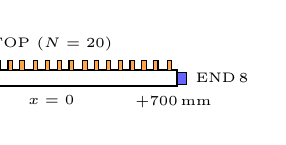
\begin{tikzpicture}[scale=0.25,trim left=-0.3cm]
  \draw[thick] (-6.4,0) rectangle (6.4, 0.8);
  \node[below,font=\tiny] at (0, 0) {$x=0$};
  \node[below,font=\tiny] at (-6.2, 0) {$-700$\,mm};
  \node[below,font=\tiny] at (6.2, 0) {$+700$\,mm};
  \foreach \xp in {-5.9,-5.2,-4.6,-4.0,-3.4,-2.8,-2.2,-1.6,-0.9,-0.3,
                   0.3,0.9,1.6,2.2,2.8,3.4,4.0,4.6,5.2,5.9} {
    \draw[fill=orange!70] (\xp, 0.8) rectangle ++(0.22, 0.5);
  }
  \node[above,font=\tiny] at (0, 1.3) {TOP ($N=20$)};
  \draw[fill=blue!60] (-6.4, 0.1) rectangle ++(-0.45, 0.6);
  \draw[fill=blue!60]  (6.4, 0.1) rectangle ++(0.45, 0.6);
  \node[left,font=\tiny] at (-6.85, 0.4) {END\,8};
  \node[right,font=\tiny] at (6.85, 0.4) {END\,8};
\end{tikzpicture}

\vspace{4pt}
{\footnotesize Orange: 20 TOP SiPMs. Blue: 8 END SiPMs/side.
$\NTOT = 36$/bar.}
\end{columns}
\end{frame}

%===============================================================================
\begin{frame}{The pooled third photon reaches 15\,ps}
\begin{columns}[T]
\column{0.50\textwidth}
\textbf{TOP $k$-scan} (EJ-230, $\NTOP=20$, $x=0$):

\vspace{4pt}
\includegraphics[width=\linewidth]{\anafig{fig1_kscan.pdf}}
\vspace{-6pt}
{\footnotesize $\sigIQR$ vs $k$. Minimum at $k^*=3$, $\sigma=15.2\ps$.}

\column{0.46\textwidth}
\textbf{Optimum and interpretation}:
\begin{itemize}
  \item $k^*=3 \Rightarrow \sigIQR(\TTOP) = 15.2\ps$
  \item $k=1$ gives $19.0\ps$ — not optimal
  \item $k>3$ averages over photons from more distant sensors
  \item \hl{$k^*=1$ is not always optimal}: the first photon may arrive from a distant SiPM and carry little timing information about the true $T_0$
\end{itemize}
\vspace{6pt}
\textbf{Train/test validation}:
\begin{itemize}
  \item Training (2500 ev): $k^*=3$, $\sigma=15.6\ps$
  \item Test (2500 ev): $\sigma = 14.99 \pm 0.38\ps$
  \item No evidence of over-fitting; global estimator is stable
\end{itemize}
\end{columns}
\end{frame}

%===============================================================================
\begin{frame}{Why did TOP improve from $\sim\!70\ps$ to $15\ps$?}
\begin{columns}[T]
\column{0.50\textwidth}
\textbf{Historical legacy result}:

\quad EJ-230 TIR, $N=70$ SiPMs, per-SiPM mean estimator:
\[
  \sigma_{\mathrm{TOP}}^{\mathrm{old}} \approx 70\ps
\]
Per-SiPM mean = average of first-photon arrival per SiPM, then average over SiPMs.

\vspace{6pt}
\textbf{Same events, same $N=20$ SiPMs, $x=0$}:
\begin{itemize}
  \item Per-SiPM mean estimator: $\sigma = 55\ps$
  \item Pooled $k=1$: $\sigma = 19.0\ps$
  \item Pooled $k^*=3$: $\sigma = 15.2\ps$
  \item \textbf{Improvement: $\times 3.6$}
\end{itemize}

\column{0.46\textwidth}
\includegraphics[width=\linewidth]{\anafig{figH_estimator_compare.pdf}}
\vspace{-4pt}
{\footnotesize Same events, same SiPMs, $x=0$, EJ-230 $N=20$.
Dashed line: per-SiPM mean ($55\ps$).
Curve: pooled $k$-th order statistic.}

\begin{alertblock}{Conclusion}
The $70\ps\to15\ps$ improvement is primarily
an \textbf{estimator advance}: pooled $k$-th vs
per-SiPM mean (same events, same SiPMs).
\end{alertblock}
\end{columns}
\end{frame}

%===============================================================================
\begin{frame}{Timing distributions: END nearly Gaussian, TOP/BLUE have tails}
\begin{columns}[T]
\column{0.97\textwidth}
\includegraphics[width=0.88\linewidth]{\anafig{figA_residuals.pdf}}
\end{columns}
{\scriptsize
$\sigIQR=(Q_{75}-Q_{25})/1.349$.
\textbf{END}: 53.7\ps\ ($p=0.09$).
\textbf{TOP}: 15.2\ps\ ($p=0.19$).
\textbf{BLUE}: 15.2\ps\ ($p=0.005$, non-Gaussian $\Rightarrow$ use $\sigIQR$).
}
\end{frame}

%===============================================================================
\begin{frame}{BLUE: minimum-variance combination}
\begin{columns}[T]
\column{0.52\textwidth}
Define two calibrated estimators $\TEND$, $\TTOP$ for the same event time $T_0$.
\[
  \Tblue = \wend\,\TEND + \wtop\,\TTOP, \quad \wend+\wtop=1
\]
Covariance matrix:
\[
  C = \begin{pmatrix}
    \sigma_E^2 & \mathrm{Cov} \\ \mathrm{Cov} & \sigma_T^2
  \end{pmatrix}
\]
BLUE weights (minimum variance, linear, unbiased):
{\small\[
  \vec w = \frac{C^{-1}\mathbf{1}}{\mathbf{1}^TC^{-1}\mathbf{1}},\quad
  \sigma_{\mathrm{BLUE}}^2 = \frac{1}{\mathbf{1}^TC^{-1}\mathbf{1}}
\]}
{\small\[
  \wend = \frac{\sigma_T^2 - C_{ET}}{\sigma_E^2+\sigma_T^2-2C_{ET}}
\]}

\column{0.44\textwidth}
\textbf{Physical interpretation}:
BLUE weights each estimator by its precision
\emph{after} accounting for correlations.

\vspace{6pt}
\textbf{At $\NTOP=20$, $x=0$}:
\begin{itemize}
  \item $\sigma_E = 53.7\ps$, $\sigma_T = 15.2\ps$
  \item $\rhoET = 0.16$ (non-negligible)
  \item $\wend = 0.013$, $\wtop = 0.987$
  \item $\sigIQR(\Tblue) = 15.2\ps$
\end{itemize}

\begin{block}{Key message}
At $\NTOP=20$: $\wend\approx1\%$,
$\sigma_{\mathrm{BLUE}} \approx \sigma_{\mathrm{TOP}} \approx 15\ps$.
\end{block}
\end{columns}
\end{frame}

%===============================================================================
\begin{frame}{$\NTOP$ scan: BLUE collapses onto TOP}
\begin{columns}[T]
\column{0.50\textwidth}
\includegraphics[width=\linewidth]{\anafig{fig_ntop_scan_full.pdf}}
\vspace{-4pt}
{\footnotesize Top: $\sigIQR$ vs $\NTOP$ for EJ-230, $x=0$.
Bottom: $\wend$ and $\rhoET$ vs $\NTOP$.}

\column{0.46\textwidth}
{\scriptsize
\begin{tabular}{rrrrrr}
\toprule
$N_T$ & $\sigma_E$ & $\sigma_T$ & $\rho$ & $w_E$ & $\sigma_B$ \\
      & [ps] & [ps] & & & [ps] \\
\midrule
4  & 51.0 & 78.2 & .15 & .74 & 45.5 \\
8  & 50.2 & 32.0 & .18 & .21 & 28.9 \\
14 & 51.0 & 18.7 & .18 & .02 & 18.2 \\
20 & 53.7 & 15.2 & .16 & .01 & 15.2 \\
\bottomrule
\end{tabular}}

\vspace{6pt}
\begin{itemize}
  \item At $\NTOP = 4$: END contributes $74\%$; BLUE genuinely combines both
  \item At $\NTOP = 14$: END contributes $<2\%$
  \item At $\NTOP = 20$: BLUE $\equiv$ TOP
\end{itemize}
\begin{alertblock}{}
This is a \emph{success} of BLUE, not a failure:\\
the estimator correctly identifies which measurement is more precise.
\end{alertblock}
\end{columns}
\end{frame}

%===============================================================================
\begin{frame}{Position dependence: resolution follows nearest TOP sensor}
\begin{columns}[T]
\column{0.50\textwidth}
\includegraphics[width=\linewidth]{\anafig{fig3_sigma_vs_x.pdf}}
\vspace{-6pt}
{\footnotesize $\sigIQR$ vs muon position $x$ for EJ-230, $\NTOP=20$.
BLUE (green, error bars) and END alone (blue dashed).
Constant fit to BLUE shown; $\chi^2/\mathrm{ndf}$ tests uniformity.}

\column{0.46\textwidth}
\textbf{Summary}:
\begin{itemize}
  \item $\sBLUE$ ranges $15$--$23\ps$ (global $k^*=3$, $m^*=8$)
  \item Peak-to-peak variation $\sim\!50\%$
  \item Positions between TOP sensors (x$=$±200, ±500) give $\sigma\approx 23\ps$
  \item Near-sensor positions give $\sigma\approx 15\ps$
\end{itemize}

\vspace{4pt}
\textbf{TOP timing bias} (relative to $x=0$):
\begin{itemize}
  \item END bias: $<15\ps$, nearly flat
  \item TOP bias: $0$ to $-104\ps$, position-dependent
  \item Discrete levels (3 groups by nearest-SiPM distance)
  \item TOP needs \hl{position-dependent calibration}
\end{itemize}

\vspace{4pt}
{\footnotesize [See backup: figE\_bias\_vs\_x]}
\end{columns}
\end{frame}

%===============================================================================
\begin{frame}{What does END provide? Timing vs position}
\begin{columns}[T]
\column{0.50\textwidth}
\textbf{END timing resolution} (hybrid geometry):
\[
  \sEND \approx 53.7 \pm 0.9\ps \quad (m^*=8)
\]
Weight in BLUE at $\NTOP=20$: $\wend \approx 1\%$.\\
\textbf{END is nearly useless for event time at $\NTOP=20$.}

\vspace{6pt}
\textbf{END position resolution}:
\[
  \sigma_x^{\mathrm{END}} \approx 7.9\mm \;(m=8)
  \quad \text{or} \quad 7.2\mm \;(m=26)
\]

\textbf{TOP centroid position} ($N_{\mathrm{pe}}$-weighted):
\begin{itemize}
  \item Bias-calibrated: $\sigma_x \approx 8$--$11\mm$
  \item Comparable to END ($7$--$8\mm$)
  \item Requires offline calibration map
\end{itemize}

\column{0.46\textwidth}
\begin{alertblock}{Key finding}
At $\NTOP=20$, TOP alone provides:
\begin{enumerate}
  \item Timing: $\sigma_t \approx 15\ps$
  \item Position: $\sigma_x \approx 8$--$11\mm$ (calibrated centroid)
\end{enumerate}
END provides comparable position ($\sigma_x \approx 7$--$8\mm$)
but negligible timing contribution.
\end{alertblock}

\vspace{6pt}
\textbf{Design question}: if TOP already provides timing AND position,
can we remove END?

\vspace{4pt}
\textbf{Answer requires}: a Geant4 simulation of the
TOP-only physical geometry (END faces replaced with
optical absorber/reflector).
This changes the photon boundary condition and
cannot be inferred from software masking alone.

\textit{[TOP-only run: proposed as next step]}
\end{columns}
\end{frame}

%===============================================================================
\begin{frame}{Channel-count Pareto frontier}
\begin{columns}[T]
\column{0.50\textwidth}
\includegraphics[width=\linewidth]{\anafig{fig_pareto.pdf}}
\vspace{-4pt}
{\footnotesize Timing resolution vs total SiPM channels per bar.
Black: END-only (8 SiPMs/end $\times$ 2, $N_{\mathrm{total}}$ as shown).
Star: $m$-average point at $N=16$.
Green: BLUE hybrid (16 END + $\NTOP$ TOP, $N_{\mathrm{total}}=16+\NTOP$).}

\column{0.46\textwidth}
\textbf{Key points}:
\begin{itemize}
  \item END-only ($N=16$, $m^*=8$): $\sigma \approx 53.7\ps$
  \item BLUE $\NTOP=4$ ($N_{\mathrm{tot}}=20$): $\sigma \approx 45.5\ps$
  \item BLUE $\NTOP=8$ ($N_{\mathrm{tot}}=24$): $\sigma \approx 28.9\ps$
  \item BLUE $\NTOP=14$ ($N_{\mathrm{tot}}=30$): $\sigma \approx 18.2\ps$
  \item \hl{BLUE $\NTOP=20$ ($N_{\mathrm{tot}}=36$): $\sigma \approx 15.2\ps$}
\end{itemize}

\vspace{4pt}
Adding 20 sparse TOP sensors to 16 END sensors:
\begin{itemize}
  \item $\times 3.5$ improvement in timing
  \item $\times 2.25$ increase in channel count
\end{itemize}

\vspace{4pt}
\textbf{Note}: all END channels use pooled $k$-th estimator with best-available $k$ per geometry; all hybrid uses BLUE with global $k^*$, $m^*$.
\end{columns}
\end{frame}

%===============================================================================
\begin{frame}{Electronics jitter: how far does 15\,ps survive?}
\begin{columns}[T]
\column{0.50\textwidth}
\includegraphics[width=\linewidth]{\anafig{figG_jitter.pdf}}
\vspace{-4pt}
{\footnotesize $\sigIQR$ vs single-channel timing jitter (SPTR, rms).
EJ-230, $x=0$, $\NTOP=20$.
Independent Gaussian jitter per photon arrival.}

\column{0.46\textwidth}
\textbf{Jitter scenarios} (optical limit at 0\,ps):
{\small
\begin{tabular}{rrrr}
\toprule
Jitter & $\sigma_{\mathrm{TOP}}$ & $\sigma_{\mathrm{END}}$ & $\sigma_{\mathrm{BLUE}}$ \\
\lbrack ps\rbrack & \lbrack ps\rbrack & \lbrack ps\rbrack & \lbrack ps\rbrack \\
\midrule
0   & 15.2 & 53.7 & 15.2 \\
50  & 30.1 & 55.1 & 27.7 \\
100 & 52.3 & 56.7 & 40.4 \\
150 & 68.0 & 63.7 & 49.2 \\
200 & 84.1 & 70.5 & 57.5 \\
\bottomrule
\end{tabular}}

\vspace{6pt}
\textbf{Key observations}:
\begin{itemize}
  \item At 50\,ps jitter: TOP $\to$ 30\,ps (factor 2 degradation)
  \item At $\geq150\ps$: END becomes competitive with TOP
  \item The $k=3$ pooled estimator amplifies per-photon jitter
  \item Realistic jitter target: $<50\ps$ SPTR for $<30\ps$ event time
\end{itemize}
\end{columns}
\end{frame}

%===============================================================================
\begin{frame}{Detector-design interpretation}
\begin{columns}[T]
\column{0.48\textwidth}
\textbf{What we know from this analysis}:

\begin{enumerate}
  \item TOP ($\NTOP=20$) gives $\sigma_t \approx 15\ps$ and $\sigma_x \approx 9\mm$
  \item END adds $<1.3\%$ weight to event time at $\NTOP=20$
  \item END gives $\sigma_x \approx 7$--$8\mm$ — comparable to TOP
  \item TOP has strong position-dependent timing bias; requires calibration
  \item At $\geq 50\ps$ channel jitter, TOP degrades significantly
  \item Uniformity: $\sigma_{\mathrm{BLUE}}$ varies 15--23\,ps with position (50\% peak-peak)
\end{enumerate}

\column{0.48\textwidth}
\textbf{Open questions}:

\begin{itemize}
  \item \textbf{TOP-only geometry}: does removing END physically change the $15\ps$ result?
    (boundary conditions change; needs new Geant4 run)
  \item \textbf{Optimal TOP layout}: uniform spacing may not minimise worst-case $\sigma_t(x)$
  \item \textbf{Common clock jitter}: separate from per-channel SPTR; needs detector-level study
  \item \textbf{TOP-alone position}: 8--11\,mm adequate? Or do we need END for $<8\mm$?
\end{itemize}

\vspace{4pt}
\begin{alertblock}{Current recommendation}
Keep $\NTOP=20$ hybrid pending TOP-only Geant4 result.
If TOP-only gives equivalent timing, 16 END channels
per bar ($\times 600$ bars $=$ 9600 channels) can be eliminated.
\end{alertblock}
\end{columns}
\end{frame}

%===============================================================================
\begin{frame}{Conclusions}
\begin{enumerate}
  \setlength\itemsep{6pt}

  \item \textbf{First principles explain the optical transport}\\
    TIR geometry, Vikuiti reflector losses, and scintillation kinetics
    correctly predict the scale and material ordering of Geant4.
    The effective PDE in simulation ($\approx0.61$) is higher than the
    original napkin assumption ($0.40$); the updated napkin gives
    $\sim\!10\%$ agreement with Geant4.

  \item \textbf{The estimator choice dominates timing performance}\\
    A pooled $k$-th order statistic on TOP outperforms the legacy
    per-SiPM mean estimator by a factor $\times 3.6$ on the same events.
    The $k^*=1$ first-photon is not optimal; $k^*=3$ gives $15.2\ps$.

  \item \textbf{At $\NTOP=20$, TOP dominates event time; BLUE $\equiv$ TOP}\\
    BLUE assigns $<1.3\%$ weight to END ($\wend=0.013$). Within
    statistical uncertainty, $\sBLUE \approx \sTOP \approx 15\ps$.
    Global (train/test) and oracle estimators agree to $<0.4\ps$.

  \item \textbf{The remaining problem is detector-level}\\
    Position-dependent TOP timing bias ($\leq104\ps$) requires calibration.
    Uniformity is $\pm50\%$ peak-to-peak along the bar.
    Electronics jitter $\gtrsim 50\ps$ degrades TOP to $>30\ps$.
    The value of END depends on the TOP-only physical geometry —
    a targeted Geant4 run is the critical next step.
\end{enumerate}
\end{frame}

%===============================================================================
\appendix
%===============================================================================

\begin{frame}
\begin{center}
  \large Backup slides
\end{center}
\end{frame}

%===============================================================================
\begin{frame}{Train/test split and oracle comparison}
\begin{columns}[T]
\column{0.50\textwidth}
\textbf{Methodology} (to avoid optimistic bias):
\begin{enumerate}
  \item Split 5000 events 50/50 by random permutation (seed 20260820)
  \item Training half: find $k^*, m^*$ by minimising $\sigIQR$
  \item Test half: apply global $k^*, m^*$ without re-optimising
\end{enumerate}

\column{0.46\textwidth}
\textbf{Results at $x=0$, EJ-230, $\NTOP=20$}:
{\small
\begin{tabular}{lrr}
\toprule
Mode & $k^*$ & $\sigma_{\mathrm{BLUE}}$ \\
\midrule
Oracle (same-sample) & 3 & $15.21\ps$ \\
Global (train/test)  & 3 & $14.85 \pm 0.40\ps$ \\
\midrule
Difference & — & $0.36\ps$ \\
\bottomrule
\end{tabular}}

\vspace{6pt}
The oracle optimistic bias is $<0.4\ps$, well within bootstrap uncertainty.
Both oracle and global agree on $k^*=3$.
\end{columns}
\end{frame}

%===============================================================================
\begin{frame}{$\rho_{\mathrm{ET}}$ and BLUE weights vs position}
\includegraphics[width=0.55\linewidth]{\anafig{figF_rho_vs_x.pdf}}
\hfill
\begin{minipage}{0.42\linewidth}
\textbf{Key findings}:
\begin{itemize}
  \item $\rhoET$ varies from $0.07$ to $0.16$ across the bar
  \item Not constant with $x$ — correlation depends on the local photon geometry
  \item $\wend$ follows $\sigma_T(x)$: where TOP is worse, END gets more weight
  \item At positions between TOP sensors (high $\sigma_T$), $\wend$ increases to $\sim 10\%$
\end{itemize}
The BLUE weights are computed position-by-position from training data.
\end{minipage}
\end{frame}

%===============================================================================
\begin{frame}{$\sigma_x^{\mathrm{END}}$ vs $m$: timing vs position}
\includegraphics[width=0.55\linewidth]{\anafig{figC_sigma_x_end.pdf}}
\hfill
\begin{minipage}{0.42\linewidth}
\begin{itemize}
  \item Left: $\sigIQR(\TEND)$ vs $m$ (timing)
  \item Right: $\sigma_x^{\mathrm{END}}=(v_{\mathrm{eff}}/2)\sigIQR(\Delta t_m)$
  \item Timing opt: $m^*=8$, $\sigma_T=53.7\ps$, $\sigma_x=7.9\mm$
  \item Position opt: $m=26$, $\sigma_x=7.2\mm$
  \item Difference $0.7\mm$: use $m=8$ for both
\end{itemize}
\end{minipage}
\end{frame}

%===============================================================================
\begin{frame}{TOP position estimators}
\includegraphics[width=0.55\linewidth]{\anafig{figD_top_position.pdf}}
\hfill
\begin{minipage}{0.42\linewidth}
\textbf{Simple TOP position estimators}:
\begin{itemize}
  \item \textbf{Earliest-hit SiPM}: discrete, bias $\leq25\mm$
  \item \textbf{$N_{\mathrm{pe}}$ centroid}: $\sigma_x\approx8$--$11\mm$ (calibrated)
  \item Uncorrected centroid bias $\leq300\mm$ (centre pull)
  \item Cal: $x_{\mathrm{est}}=f(\mathrm{centroid})$ from training data
\end{itemize}
\vspace{4pt}
Horizontal dashes: END position resolution at $m=m^*=8$ ($\sigma_x\approx7.9\mm$).
END and TOP centroid give comparable position resolution.
\end{minipage}
\end{frame}

%===============================================================================
\begin{frame}{Electronics jitter — detail}
\includegraphics[width=0.55\linewidth]{\anafig{figG_jitter.pdf}}
\hfill
\begin{minipage}{0.42\linewidth}
{\small
\textbf{Jitter model}:
\begin{itemize}
  \item Gaussian SPTR per photon, independent
  \item $t_i \to t_i + \mathcal{N}(0,\sigma_j^2)$, re-sort
  \item Scenario study (not measured)
\end{itemize}
\textbf{Physical interpretation}:
\begin{itemize}
  \item TOP: $k$-th photon displaced by jitter
  \item END $m$-avg: jitter reduced by $\sqrt{m}$
  \item $\sigma_j=150\ps$: END $\approx$ TOP
\end{itemize}
}
\end{minipage}
\end{frame}

%===============================================================================
\begin{frame}{PDE audit and napkin photon budget}
\begin{columns}[T]
\column{0.50\textwidth}
\textbf{Simulation PDE} (AFBR-S4N66P024M, from data):
\begin{itemize}
  \item Mean PDE (all detected photons): $0.607$
  \item Range: $0.00$--$0.63$ (wavelength-dependent)
  \item No significant difference between END and TOP faces
\end{itemize}

\column{0.46\textwidth}
\textbf{Updated napkin} (EJ-230, per end, PDE$=0.61$):
\[
  N_{\mathrm{pe}}^{\mathrm{napkin}} \approx 1275 \times 0.61 \approx 778\,\mathrm{pe/end}
\]
vs Geant4: $\approx 701\,\mathrm{pe/end}$.

Agreement at $\sim\!10\%$ — better than with PDE$=0.40$ ($\sim\!40\%$ low).
\end{columns}

\vspace{8pt}
\begin{block}{Corrected photon-budget comparison (per end)}
\centering
\begin{tabular}{lrr}
\toprule
Quantity & Napkin & Geant4 \\
\midrule
$N_\gamma$ produced & 19\,400 & — \\
$f_{\mathrm{TIR,end}}$ & 0.274 & — \\
$P_{\mathrm{surv}} \times$ coverage & $\sim 0.50 \times 0.48$ & — \\
PDE & 0.61 & 0.61 (measured) \\
$N_{\mathrm{pe}}$/end & $\approx 778$ & $\approx 701$ \\
\midrule
Agreement & \multicolumn{2}{c}{$\approx\!10\%$} \\
\bottomrule
\end{tabular}
\end{block}
\end{frame}

%===============================================================================
\begin{frame}{Proposed next Geant4 run: TOP-only geometry}
\textbf{Motivation}: at $\NTOP=20$, BLUE gives $\wend \approx 1\%$.
Can the 16 END channels be eliminated?

\vspace{6pt}
\textbf{What cannot be inferred from existing data}:
\begin{itemize}
  \item Removing END SiPMs changes the optical boundary condition at the end faces
  \item Photons that currently enter END SiPMs would instead be reflected/absorbed
  \item This modifies the photon population reaching TOP SiPMs
  \item The effect on $\sigma_t^{\mathrm{TOP}}$ is unknown without a physical simulation
\end{itemize}

\vspace{6pt}
\textbf{Proposed run}:
\begin{itemize}
  \item Same bar, same Vikuiti wrapping, same $\NTOP=20$ positions
  \item End faces: replace SiPMs with physical reflector or absorber
  \item Same muon scan (all 13 $x$ positions), 5000 events each
  \item Apply same pooled-$k$ estimator; compare with hybrid result
\end{itemize}

\vspace{6pt}
\textbf{Expected outcome}: if TOP-only gives $\sigma_t \approx 15\ps$ and $\sigma_x \approx 10\mm$,
then 16 END channels/bar ($\times600$ bars $= 9600$ channels) can be eliminated from the full detector.
\end{frame}

\end{document}
